\providecommand{\relativeRoot}{../..}
\documentclass[\relativeRoot/main.tex]{subfiles}
\graphicspath{{\subfix{./figures/}}}


\begin{document}

\section{Implementation}
\label{sec:lyprox:implementation}

\subsection*{Database models}
\label{subsec:lyprox:implementation:models}

\begin{figure}
    \centering
    \def\svgwidth{1.0\textwidth}
    \input{figures/er_diagram_paths.pdf_tex}
    \caption[
        ER diagram of LyProX' data model
    ]{
        \Gls{er} diagram of LyProX' underlying data representation. Every box corresponds to one Python \texttt{class} in Django and therefore also to one table in the SQLite3 database. Entries in those tables are linked to other table's entries via the indicated connections. The connections between nodes of this graph are all \emph{one-to-many} relations, meaning that e.g. one institution per user, but many users per institution.
    }
    \label{fig:lyprox:er_diagram}
\end{figure}

The first step in creating a Django web application -- aside from initializing the project by choosing important settings -- usually consists of defining the database models. This is done by writing a Python class -- inheriting from Django's \texttt{Model} class -- for each type of object one wants to store. One such class essentially corresponds to a table in the underlying database (e.g., an \acrshort{sql} database like \href{https://www.sqlite.org/index.html}{SQLite3}). It can be given attributes for each column in that table and may also store relationships between tables/classes. Based on this Python representation of data, Django can automatically create extensive functionality. As their documentation states: 

\begin{displayquote}[Django documentation \cite{noauthor_creating_nodate}]
    The goal is to define your data model in one place and automatically derive things from it.
\end{displayquote}

For example, when we defined the \texttt{Patient} class, we used Django to generate large parts of the utilities that render \acrshort{html} forms for creating, editing and deleting \texttt{Patient} entries in the respective SQLite3 database. In total, we created six entities to represent our patient cohorts in the database:

\begin{itemize}
    \item \texttt{Insitution:} Represents a hospital or medical research facility that has created datasets of patients, e.g. from their treatment records.
    \item \texttt{User:} A member of one of the \texttt{Institutions} who uploaded data into the web page's database or whom we granted access to those \texttt{Datasets} we did not yet make public.
    \item \texttt{Dataset:} Groups \texttt{Patients} into cohorts that were extracted or added to the interface at the same time. This entity stores additional information such as the repository it is made persistent in -- if available -- or whether it is public. We implemented this last property to be able to visualize progression patterns of patients that are not yet ready for publication.
    \item \texttt{Patient:} The core entity in the database corresponding to a patient record. It encodes e.g. demographic information such as age and sex, as well as TNM stage. It belongs to a \texttt{Dataset} and can hold multiple \texttt{Tumors} and \texttt{Diagnoses}.
    \item \texttt{Tumor:} We could have added information about the primary tumor directly to the \texttt{Patients} table, but at some point we might want to be able to deal with multiple synchronous tumors. Due to this potential extension in the future, we created a separate entity for tumors and allow a \texttt{Patient} to be associated with multiple tumors. It stores tumor-specific data, such as its location, lateralization and volume -- if available.
    \item \texttt{Diagnose:} For the reporting of \acrlong{lnl} involvement, this is the Django \texttt{class} of interest. For each side of a \texttt{Patient's} neck (ipsi- and contralateral) and for each modality that reported lymphatic involvement (e.g. \gls{mri}, \gls{ct}, pathology, ...), one such entry exists. It stores whether each \gls{lnl}'s state was reported to be metastatic, healthy or unknown. For example, \glspl{fna} are usually only performed for one or two levels at a time. All other levels would then be empty in the respective \texttt{Diagnose} entry.
\end{itemize}

A detailed \gls{er} diagram is shown in \cref{fig:lyprox:er_diagram}. It also lists all attributes that are stores for each entity and what Django type is used to represent them.

\subsection*{Adding patients}
\label{subsec:lyprox:implementation:add}

\begin{figure}
    \centering
    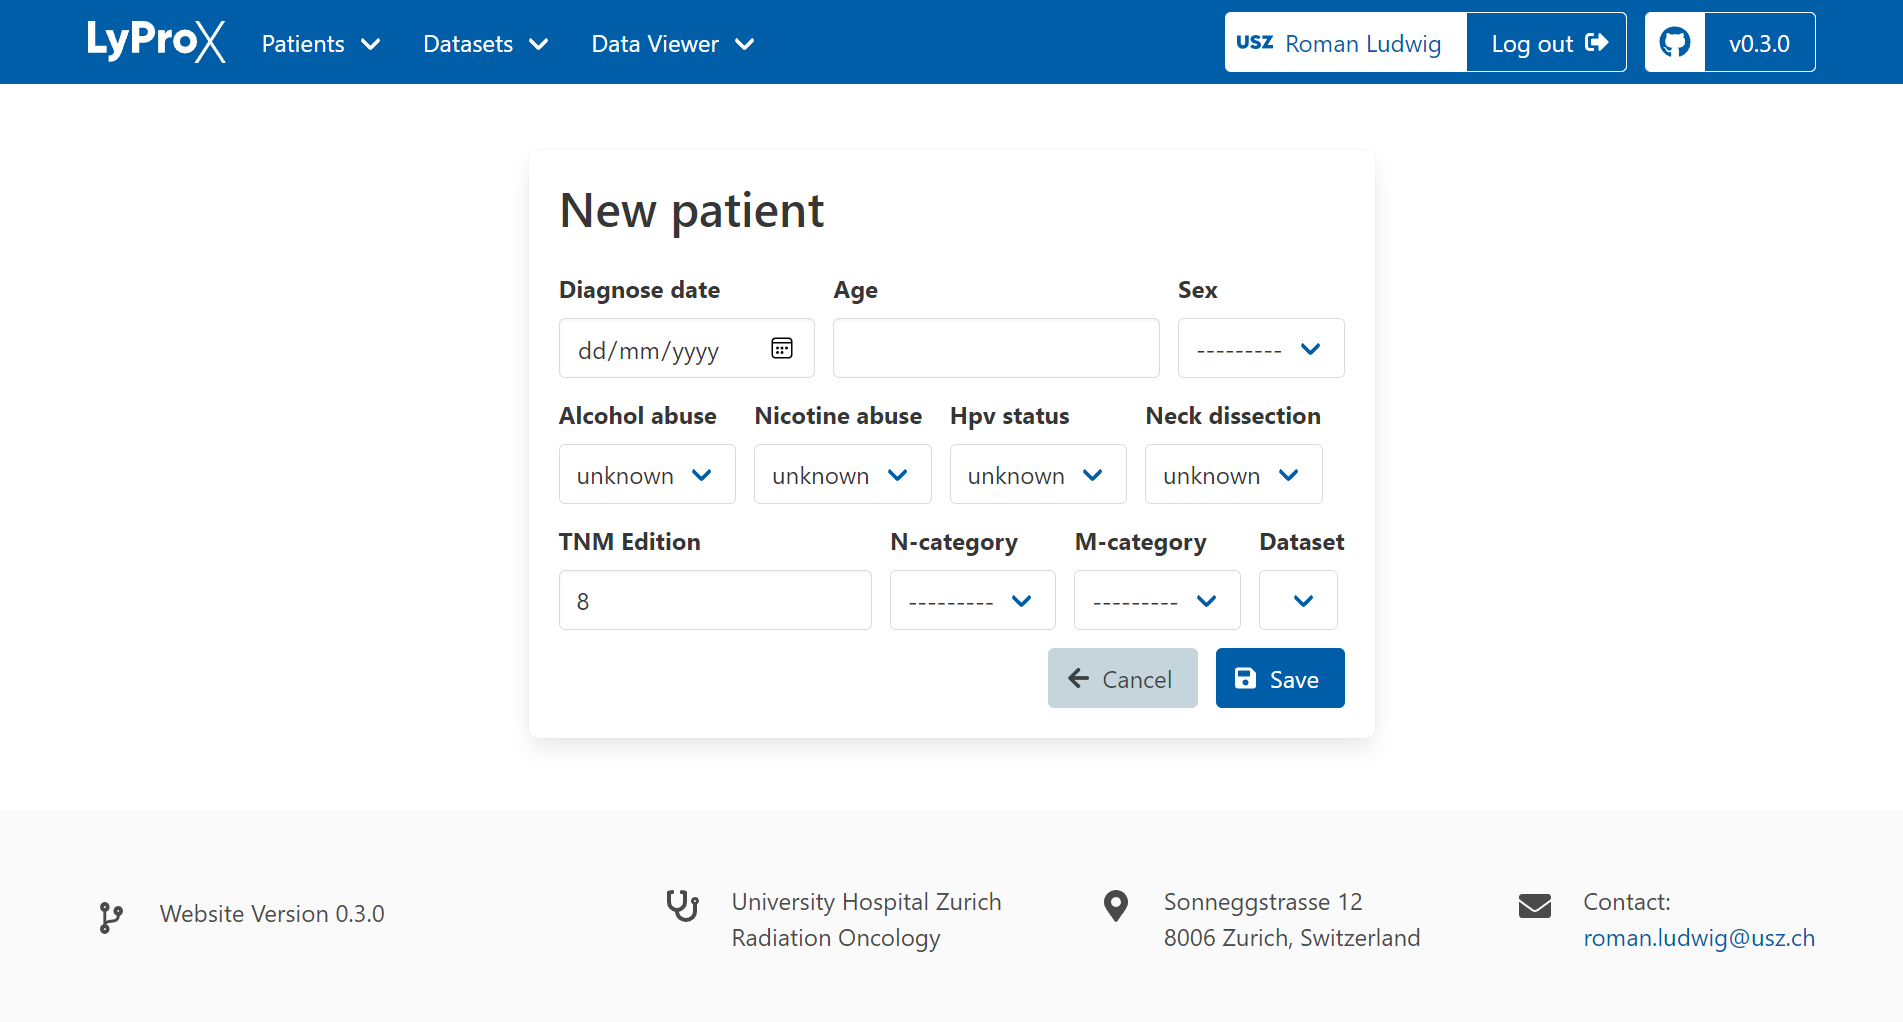
\includegraphics[width=1.0\textwidth, frame]{figures/new_patient.png}
    \caption[
        Screenshot of the form for adding new patients
    ]{
        Screenshot of the rendered \acrshort{html} form that is shown when an authenticated user wants to add a new \texttt{Patient} to an existing \texttt{Dataset}. Note that the form contains no field for specifying a T-stage.
    }
    \label{fig:lyprox:new_patient}
\end{figure}

As mentioned earlier, Django's design principles allow developers to reuse as much as possible of already written code. Hence, most of the functionality to add, edit or delete any of the just introduced database entities was already implemented. Django does this via \texttt{Form} classes that are built around the user-created \texttt{Model} classes. Those Django forms can then in turn render \acrshort{html} forms into which a user can enter data that -- when sent back to the server -- will be translated by the same \texttt{Form} class into a new or changed database entry.

On top, one may implement custom logic to sanitize a user's input or derive \texttt{Model} attributes from inputs. An example in LyProX would be the T-stage: As shown in \cref{fig:lyprox:er_diagram}, for every \texttt{Patient}, we store the attribute \texttt{t\_stage}. But when creating a new patient (see screenshot in \cref{fig:lyprox:new_patient}), there is no field for T-stage. After the new \texttt{Patient} entry has been created, however, one may add a \texttt{Tumor} to it, for which a T-stage must be defined. Upon writing the tumor information into the database, Django calls a method in the \texttt{Patient} class updating this instance's T-stage to be the most advanced of all its tumors (see \cref{fig:lyprox:sanitize_t_stage}).

\begin{figure}
    \centering
    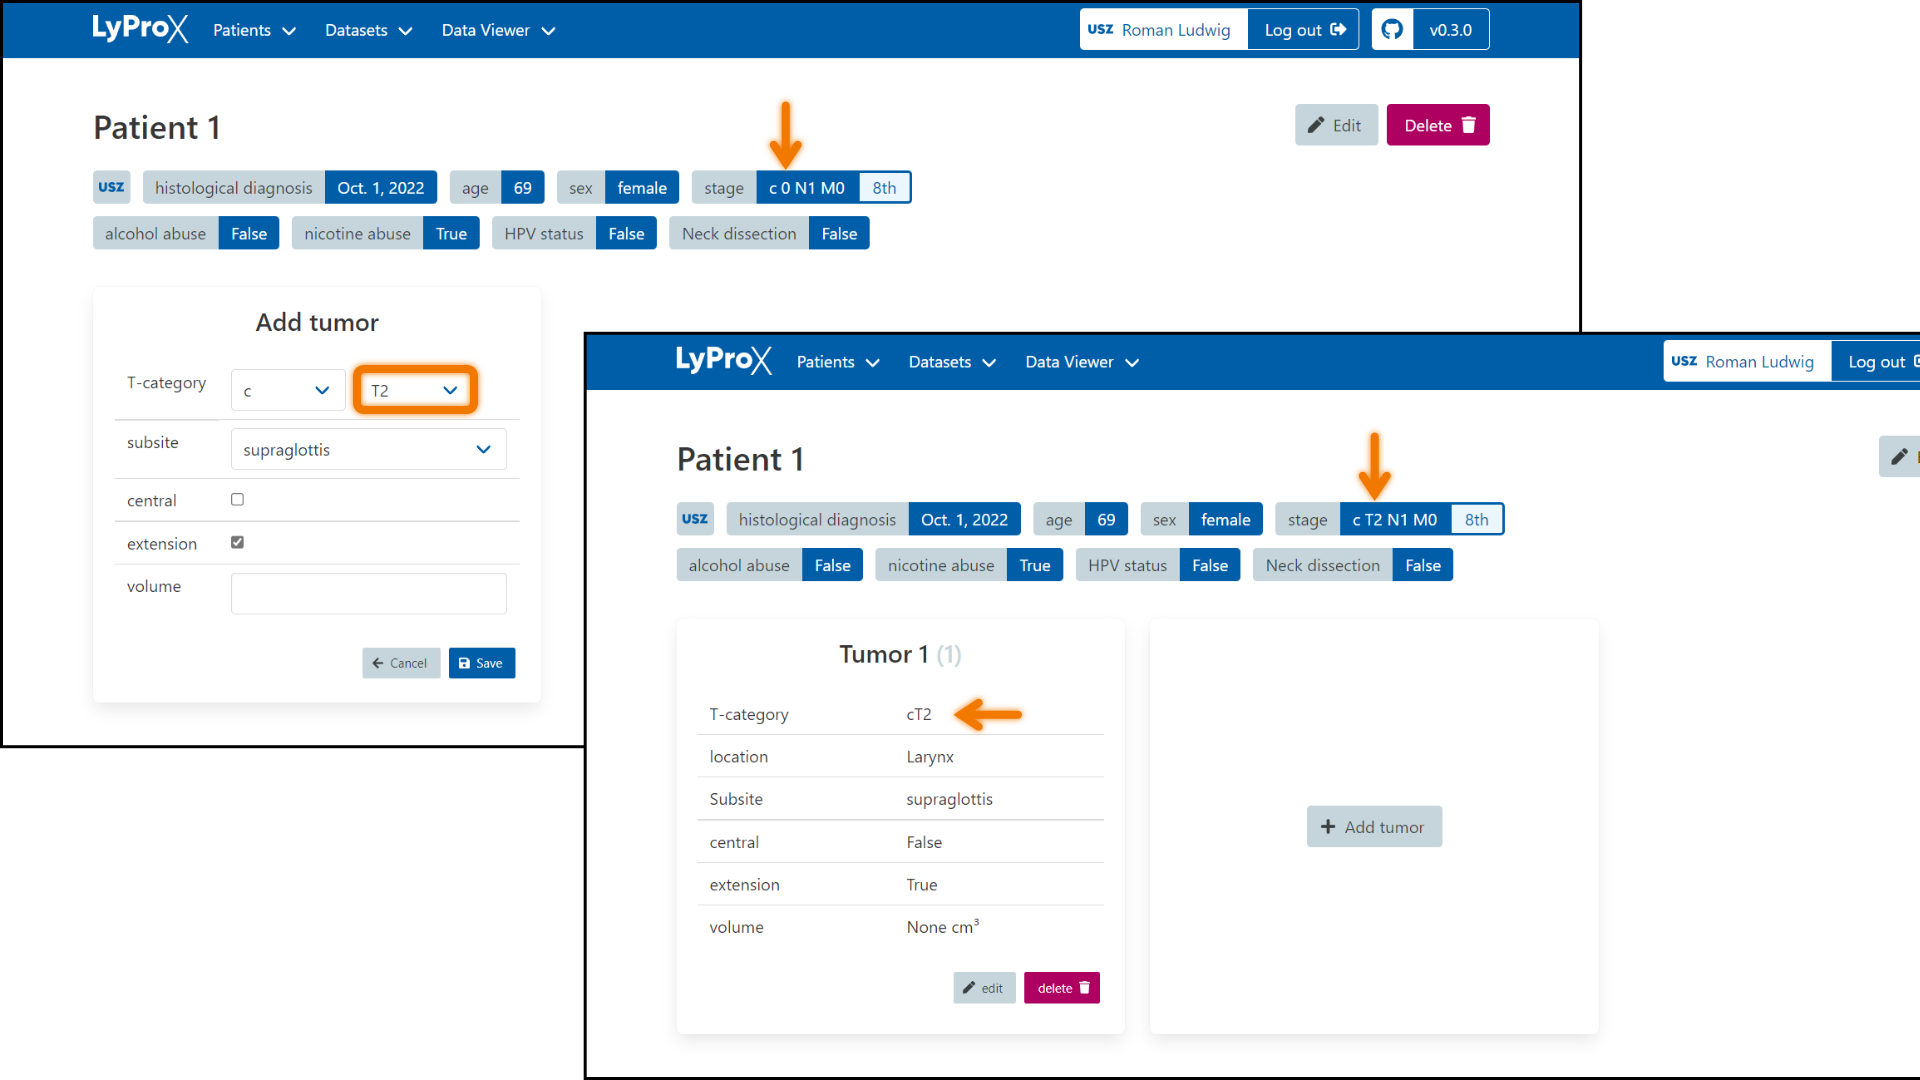
\includegraphics[width=1.0\textwidth]{figures/sanitize_t_stage.png}
    \caption[
        Process of adding a new tumor to a patient
    ]{
        Screenshot of the page displaying the newly created patient where information about the primary tumor is just being filled in (top left panel in the back), as well as a screenshot of the same patient page after the tumor was added (bottom right panel in front). The orange arrows indicate how the information is added during the process.
    }
    \label{fig:lyprox:sanitize_t_stage}
\end{figure}

Similarly, we implemented sanitization of some \glspl{lnl} in the \texttt{Diagnose}, where we need to make sure that the combination of lymphatic super- and sublevels is consistent. E.g., if we add a \texttt{Diagnose} to a \texttt{Patient} and report \gls{lnl} IIa to be healthy, but the other sublevel IIb to harbor metastases, then we automatically set the super level II to ``involved''. The other way around, when \gls{lnl} II is entered as being healthy, we can deduce that all sublevels (IIa and IIb) must be set to healthy, as well.

When one is done adding \texttt{Patient} entries to a \texttt{Datasets}, it can be locked to preserve it as created by preventing accidental edits. A method in the \texttt{Dataset's} definition is called whenever an attempt to change a \texttt{Patient}, \texttt{Tumor} or \texttt{Diagnose} is made, and raises an exception before the change can be written to the SQLite3 database.

The described implementation would in principle allow clinicians to directly transfer patient information from the digital patient record system of their insitution into LyProX. But of course most researchers do not extract lymphatic patterns of progression for the sole purpose of adding them to our interface. Hence, the definition of a \texttt{Dataset} in Django contains convenience methods to import and export all its patients from and to \gls{csv} tables. This means we can take any spreadsheet-like file, rename its column headers according to what LyProX expects and batch-import entire patient cohorts in a relatively straightforward manner.

The \gls{csv} format that is expected by LyProX is also used in the implementation of the probabilistic \repolink{lymph} model (see also  \cref{chap:unilateral}) to load the data for learning, and for publishing our raw data in \repolink{lyDATA}, where it is also described in great detail.

\subsection*{Visualizing patterns of progression}
\label{subsec:lyprox:implementation:viewer}

\begin{figure}
    \centering
    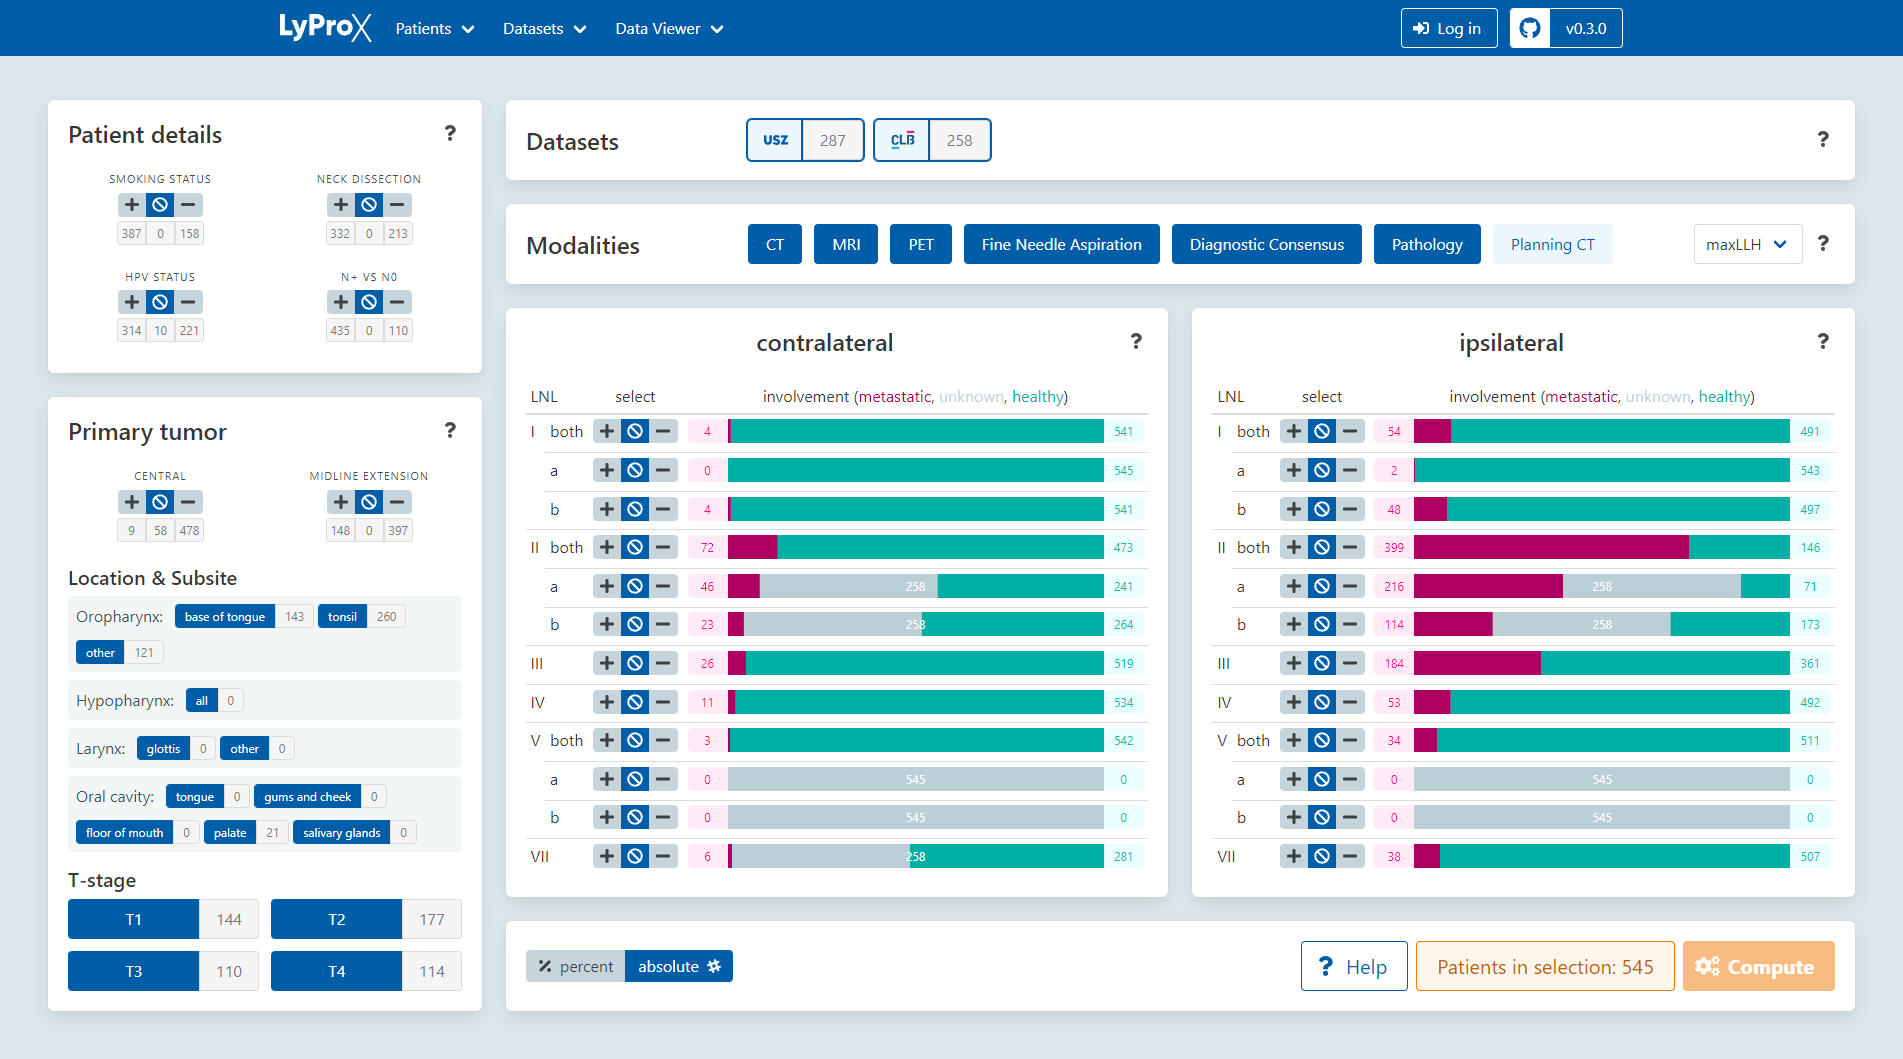
\includegraphics[width=1.0\textwidth, frame]{figures/data_viewer.png}
    \caption[
        Screenshot of the data viewer dashboard
    ]{
        A screenshot of the data viewer. Users can filter patients in the datasets by different criteria: General information, e.g. smoking status (top left box), tumor characteristics like location and T-stage (bottom left box), dataset of origin (top right bar), which reported modalities to include and how to combine them (second bar from top, right side) and finally they may be filtered by per-level involvement (two tall boxes in the right column). Controls are placed in the bottom right bar.
    }
    \label{fig:lyprox:data_viewer}
\end{figure}

The part of the \gls{gui} we originally set out to build with Django can be found in the ``Data Viewer'' tab within LyProX. At its core, the page that opens after switching to this tab is another \acrshort{html} form rendered by an extensively modified Django \texttt{Form} class.

On the front end, it contains numerous buttons and switches, most of which are versions of the \acrshort{html} elements \texttt{RadioButton} and \texttt{CheckBox}, styled with custom \acrshort{css} definitions. Of those buttons, some are what we termed \emph{three-way toggle buttons}, and they allow the user to make an optional binary choice. This means one may select ``true/positive/+'', ``false/negative/--'' or ``neutral'' where the latter corresponds to not making a choice w.r.t. this particular criterion.

\begin{samepage}
    \setlength\intextsep{0pt}
    \begin{wrapfigure}{l}{0.2\textwidth}
        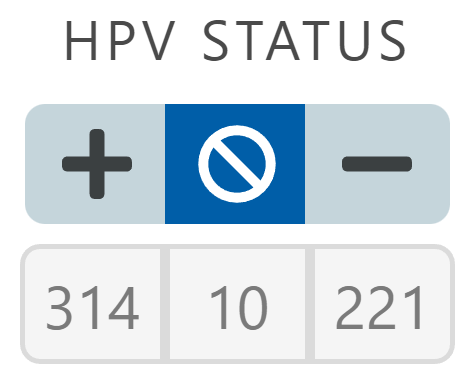
\includegraphics[width=0.18\textwidth]{figures/hpv_neutral.png}
    \end{wrapfigure}
    One such button is shown here on the left. Its switch is in the neutral middle \faIcon{ban} position, as indicated by the highlight in blue, and hence no selection is performed w.r.t. its selection criteria (\gls{hpv} status here). Below the button it shows how many patients in the current selection are \gls{hpv} positive (left number, 314 here), \gls{hpv} negative (right number, 221 here) or do not have \gls{hpv} related information available (number in the middle, 10 here).

    \begin{wrapfigure}{l}{0.2\textwidth}
        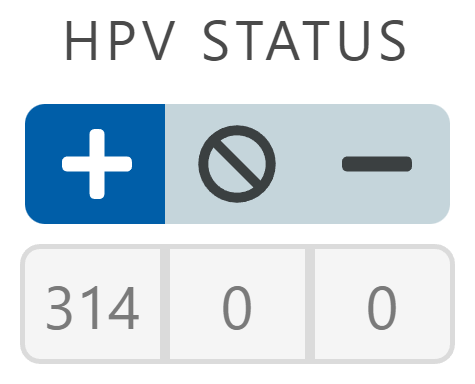
\includegraphics[width=0.18\textwidth]{figures/hpv_positive.png}
    \end{wrapfigure}
    To select all \gls{hpv}-positive patients, a user would have to click the \faIcon{plus} symbol. The highlight then switches to the left and after applying the selection (e.g. by clicking the orange ``Compute'' button that appears on the lower right side of the data viewer in \cref{fig:lyprox:data_viewer}) the numbers below the toggle button update as well: Their meaning remains the same, but since the patient selection now only contains \gls{hpv} positive patients, those that are \gls{hpv} negative or have an unknown \gls{hpv} state are filtered out.

    \begin{wrapfigure}{l}{0.2\textwidth}
        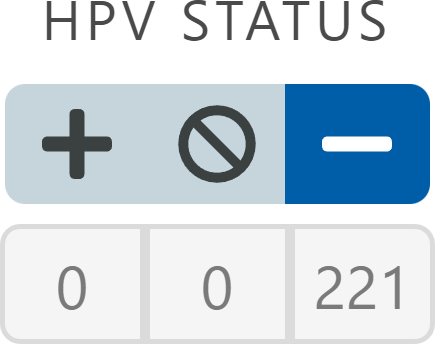
\includegraphics[width=0.18\textwidth]{figures/hpv_negative.png}
    \end{wrapfigure}
    Lastly, to keep only \gls{hpv} negative patients in the selection, the switch has to be brought into the position shown here on the left by clicking the \faIcon{minus} symbol. Again, after updating/recomputing, the only patients that remain selected are the ones that are \gls{hpv} negative.

    
\end{samepage}

As can be seen in \cref{fig:lyprox:data_viewer}, the overall layout  of the interface is divided into five blocks allowing the user to filter patients w.r.t. five different aspects:

\begin{itemize}
    \item \textbf{Patient details}~(left column, top box): Four three-way toggle buttons allow patient selection by general information: Whether patients were reported to be smokers, their treatment included a \acrlong{nd}, they were \gls{hpv} positive/negative and whether they were $N_0$ or $N_+$ patients.
    \item \textbf{Primary tumor}~(left column, bottom box): Offers selection criteria related to the tumor. Two toggle buttons allow selection w.r.t. to the lateralization (central/asymmetric and extension over the mid-sagittal plane) and multiple buttons to (de)select patient with tumors originating in various locations and subsites. Lastly in that box, one can (de)select tumors of certain T-stages.
    \item \textbf{Datasets}~(right column, top bar): In this row we list the different datasets and how many patients of each cohort are included in the selection. Here, the user can also (de)select patients from any cohort that they do (not) want to be included.
    \item \textbf{Modalities}~(right column, second bar from top): Many patients might have conflicting information on their \gls{lnl} involvement. E.g., if a \gls{ct} scan reports no involvement, but the pathologist finds microscopic metastases after a \gls{nd}. With the buttons in this bar, one can keep only those patients that have at least one of the selected modalities in their information. Conflicts are then lifted using the method chosen in the drop-down menu on the right. A basic example would be the logical OR, which we used in \cref{chap:dataset_usz}. It displays a patient's \gls{lnl} as metastatic as soon as one of the selected modalities does so. The naive maximum likelihood estimate employed in \cref{chap:dataset_clb} on the other hand considers the trustworthiness of a (diagnostic) modality based in its sensitivity and specificity (see \cref{subsec:dataset_clb:methods:max_llh} for more details).
    \item \textbf{Contra- \& ipsilateral Involvement}~(right column, two large boxes next to each other): The main information is displayed here. Within each box for the corresponding side, we display the prevalence of metastases per \gls{lnl} as observed in the set of included patients. Every level is shown in its own labelled row that is also equipped with another three-way toggle button. Setting it to \faIcon{plus} (and recomputing) causes the interface to only show patients with observed involvement in that \gls{lnl}. For example, we can check how many patients show ipsilateral \gls{lnl} IV involvement but a healhty \gls{lnl} V, by setting the button in row ``IV'' of the right box to \faIcon{plus}, and in row ``V both'' to \faIcon{minus}. Subsequently, pressing the orange ``compute'' button on the bottom right of the page displays the interface as shown in \cref{fig:lyprox:data_viewer_lnl_example}. Right next to the toggle buttons we plot how many patients in the selected cohort show involvement of the respective \gls{lnl}. It is a horizontally stacked bar plot: The red bar indicates the portion of patients with metastases in the level, the green bar the portion of those without any detected cancer and a gray bar indicates the level was not diagnosed or resected for the corresponding portion of patients.\\
    [3mm]
    \begin{tikzpicture}
        \node (image) at (0,0) {
            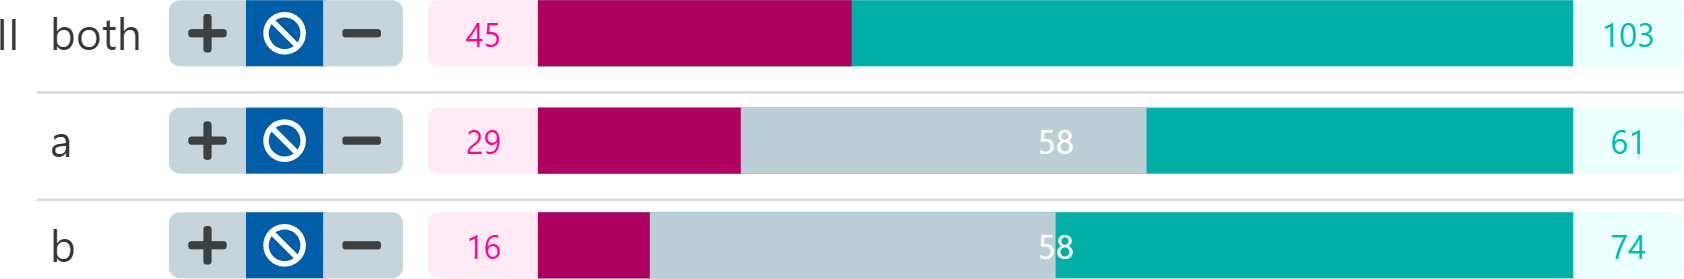
\includegraphics[width=0.92\textwidth]{figures/lnl_bar.png}
        };
        \draw[latex-, very thick, uszorange] (-6.1,1.2) -- (-5.8,1.9) node[above, uszorange]{\small LNL label};
        \draw[latex-, very thick, uszorange] (-4.47,-1.225) -- ++(0.0,-0.5) node[below, uszorange]{\small toggle button};
        \draw[latex-, very thick, uszorange] (-2.7,0.95) edge (-2.0,1.65)
        (-1.5,1.2) -- (-2.0,1.65)
        node[above, uszorange, text width=4.5cm, align=center]{\small number \& portion of patients with involvement};
        \draw[latex-, very thick, uszorange] (3.2,1.2) edge (3.7,1.65)
        (6.05,0.95) -- (3.7,1.65)
        node[above, uszorange, text width=5cm, align=right]{\small number \& portion of patients with a healthy level};
        \draw[latex-, very thick, uszorange] (1.5,-0.2) edge (0.5,-1.725)
        (0.0,-1.2) -- (0.5,-1.725)
        node[below, uszorange, text width=6cm, align=center]{\small number \& portion of patients where LNL status is unknown};
    \end{tikzpicture}\\
    [3mm]
    Above we have labelled the three rows showing the prevalence of involvement in level II contralaterally, along with that \gls{lnl}'s sublevels.
    \item \textbf{Controls}~(right column, bottom bar): In this last box we have placed a few controls: On the left, we have a normal toggle button, allowing the user to switch between percentages and absolute numbers. In case the former is selected, all patient counts in the interface will be replaced by percentages. On the right we have three buttons (from left to right): The ``\faIcon{question} Help'' button redirecting to LyProX' \href{https://lyprox/dashboard/help}{help page}, next a button displaying the total number of patients in selection and linking to a list of them, and finally the bright orange ``\faIcon{cogs} Compute'' button which needs to be pressed for the interface to update. We have considered automatically updating the dashboard after each user input, e.g. when a toggle button is switched. However, in that case the number of requests sent to the server would be much larger and the perceived responsiveness of the interface might suffer, because after each click there would be a split-second delay until all numbers and bars update.
\end{itemize}

\begin{figure}
    \centering
    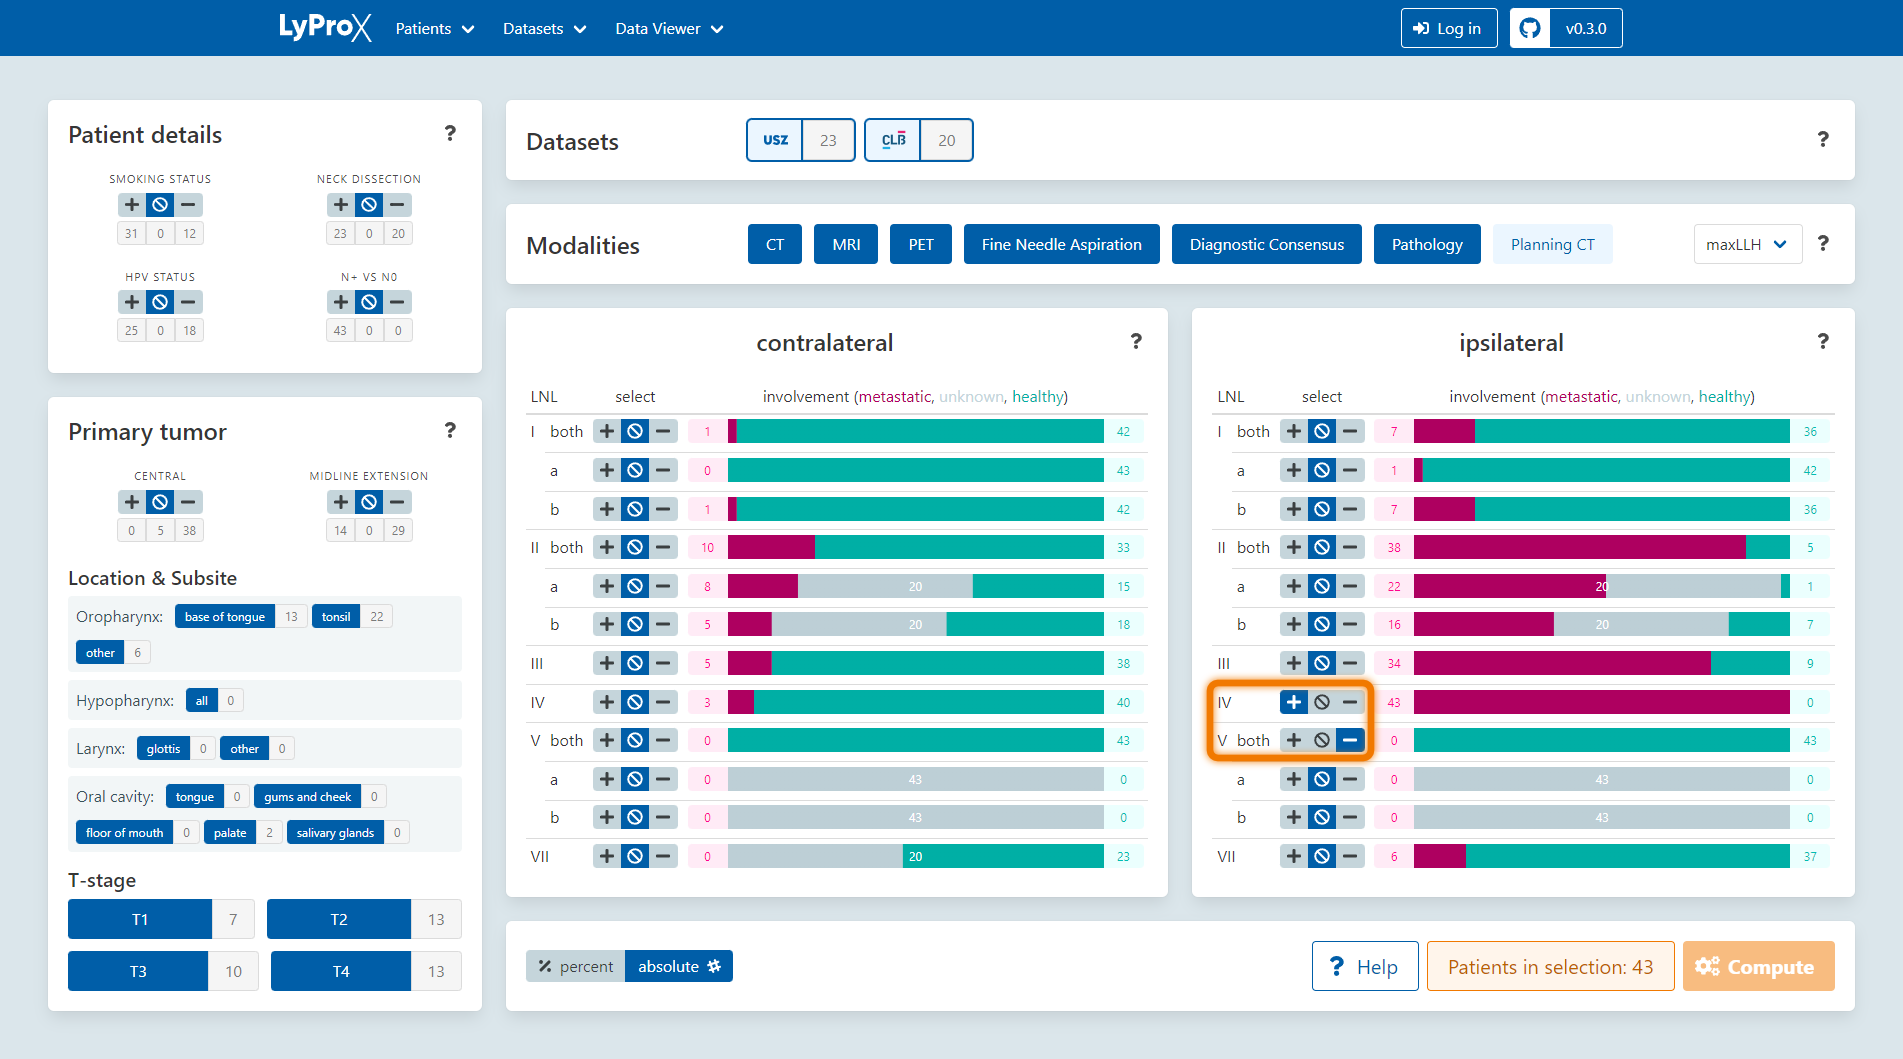
\includegraphics[width=1.0\textwidth, frame]{figures/data_viewer_lnl_example.png}
    \caption[
        The data viewer showing a scenario of two involved LNLs
    ]{
        The data viewer with the following filtering applied: It includes only patients with reported metastases (based on the consensus of selected modalities) in \gls{lnl} IV, without malignancies found in \gls{lnl} V. The three-way toggle buttons whose setting has been changed are outlined in orange.
    }
    \label{fig:lyprox:data_viewer_lnl_example}
\end{figure}

\subsection*{Styling, Layout and Design}
\label{subsec:lyprox:implementation:design}

Conceptually, the described online interface still fulfills the same purpose as the prototype shown in \cref{subsec:lyprox:motivation:prototype}. The new Django-based implementation has -- over the initial development period -- added a few more options for filtering the cohorts and how to treat multiple diagnoses per patient. Most visually striking, however, might be the overhauled visuals. The original prototype used the Python library \href{https://kivy.org}{Kivy} to run and render the \gls{gui}, which means the appearance is adjusted in the interface's code. LyProX, on the other hand, only serves \acrshort{html} pages which are styled on the client side using the \gls{css} code delivered with it. This has the disadvantage that we could not easily transfer the appearance of the prototype to the online interface, but it makes setting up a modern, responsive and professionally looking web page very straightforward: There exists an abundance of \gls{css} frameworks that provide pre-defined and carefully designed building blocks that can quickly be combined and adapted to one's needs. All we had to do is basically ship the slightly customized \gls{css} code alongside the \acrshort{html} responses to create a visually appealing \gls{gui}.

We used the popular free and open source \gls{css} framework \href{https://bulma.io}{\faIcon{external-link-alt}~Bulma} \cite{thomas_bulma_2021}, which is published under MIT license. Very little \gls{css} knowledge is required to employ it effectively, but it is still heavily customizable and extensible, making it a safe choice for further development and potential design changes in the future.

Because we find the appearance of most default Bulma elements and components very appealing, we only customized the standard colors. For those, we chose the corporate design colors of the \gls{usz}. Initially, we decided to use them because we planned to host the website under an official \gls{usz} domain and on dedicated hardware from our institution. However, the slow and bureaucratic process of our IT department forced us to host LyProX externally and under our own domain. Nonetheless, we find the \gls{usz} color scheme pleasing and modern-looking, so we kept it.

In \cref{fig:lyprox:plain_vs_bulma} we show a side-by-side comparison of a very simple \acrshort{html} page with and wihtout the custom Bulma \gls{css} we also use for LyProX. Notably, Bulma is agnostic to the type of \acrshort{html} tag. This can be seen in \cref{fig:lyprox:bulma}, where the title ``Bulma Demo'' corresponds to a normal \texttt{<p>} paragraph. Bulma's styling is always applied to class definitions of \acrshort{html} tags. In this case \texttt{<p class="title">} causes the larger font face, while the color depends on the parent \acrshort{html} element and its background color (see \cref{fig:lyprox:bulma}). This allows for a separation of form and function. E.g., a link \texttt{<a href="https://lyprox.org" class="button">} will look exactly the same as a submit button \texttt{<button type="submit" class="button">} when styled with Bulma, but might serve entirely different purposes.

\begin{figure}
    \begin{subfigure}[b]{0.48\textwidth}
        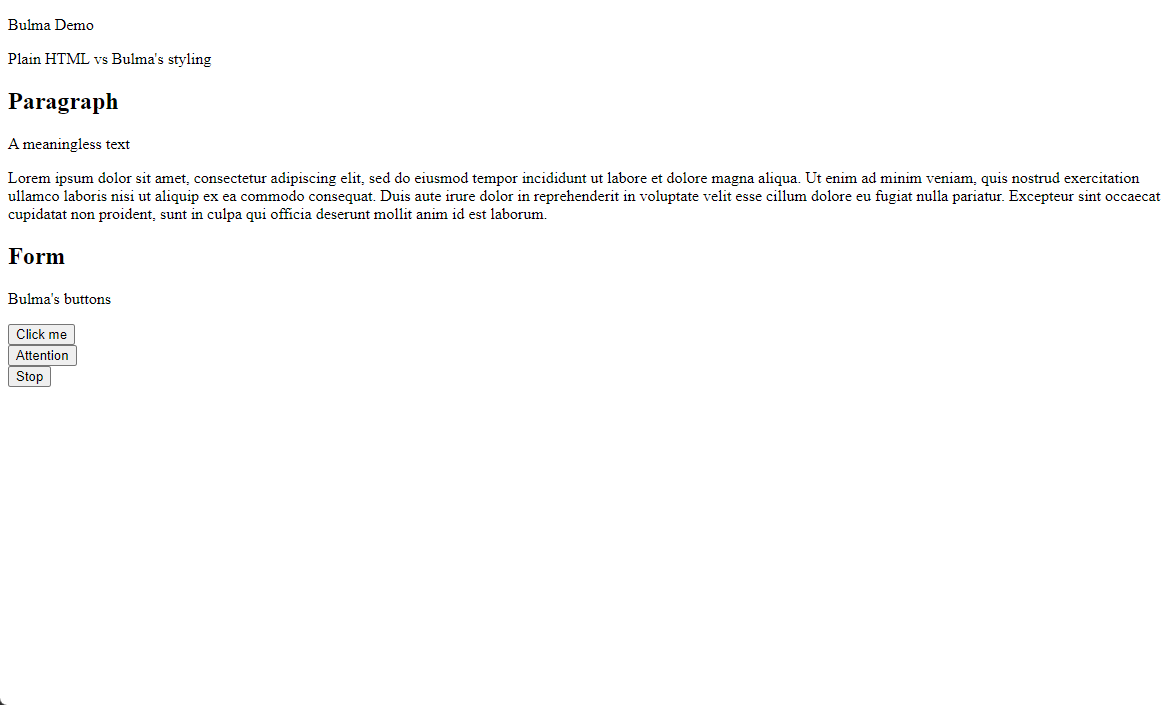
\includegraphics[width=\textwidth, frame]{figures/demo_without_bulma.png}
        \caption[
            Plain demo HTML document
        ]{
            Plain \acrshort{html} document for demonstration purposes, containing titles, a paragraph and three buttons.
        }
        \label{fig:lyprox:plain}
    \end{subfigure}
    \hfill
    \begin{subfigure}[b]{0.48\textwidth}
        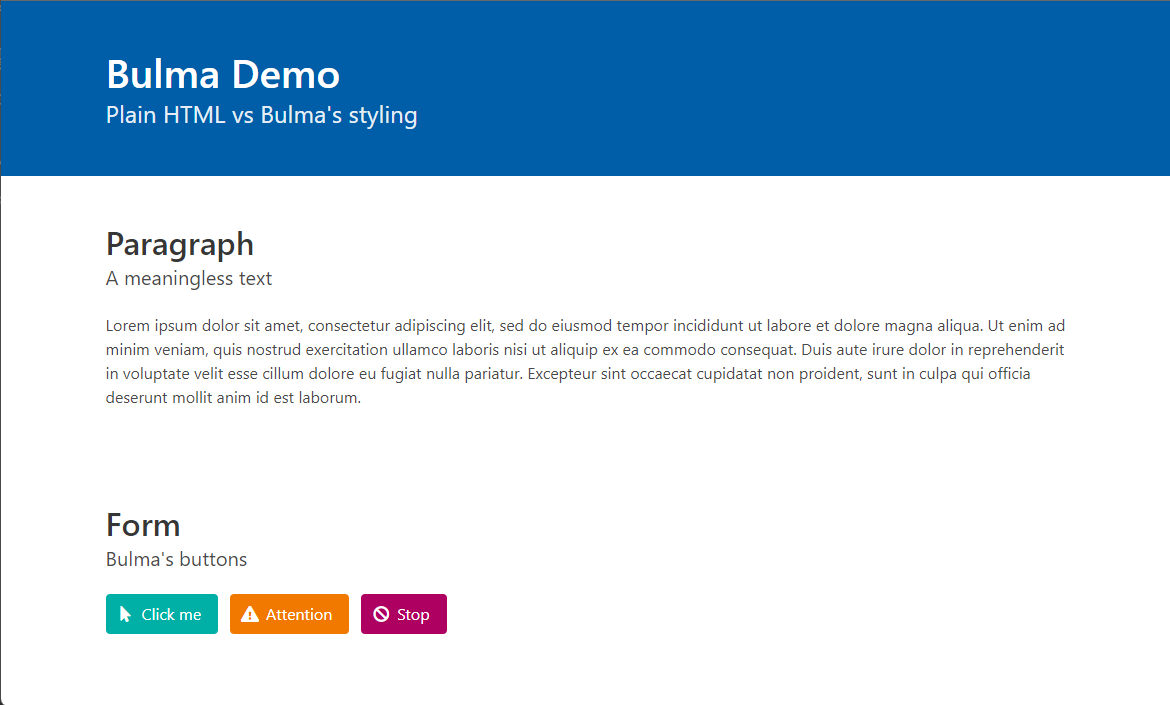
\includegraphics[width=\textwidth, frame]{figures/demo_with_bulma.png}
        \caption[
            HTML demo document with Bulma styling
        ]{
            The same \acrshort{html} document with Bulma \acrshort{css} styling with a color scheme matching the \gls{usz} corporate design.
        }
        \label{fig:lyprox:bulma}
    \end{subfigure}
    \label{fig:lyprox:plain_vs_bulma}
\end{figure}

Besides Bulma's \gls{css}, we also use \href{https://fontawesome.com}{\faIcon{font-awesome-flag}~Font Awesome Free} (version 5) \cite{noauthor_font_2022} as a provider of icons. It allows the free use of 1,608 icons under the license \faIcon{creative-commons}\faIcon{creative-commons-by} \gls{cc-by} to make interface elements more visually appealing and familiar looking. Moreover, Bulma explicitly supports adding Font Awesome icons to many of its core elements. Their icons are also used throughout this thesis to provide visual cues, e.g. in the contribution boxes.

\subsection*{Development and Deployment}
\label{subsec:lyprox:implementation:develop_deploy}

LyProX' source code is developed under MIT license in a \faIcon{git-alt}~git \cite{torvalds_git_2022} repository that is publicly hosted on \href{https://github.com/rmnldwg/lyprox}{\faIcon{github}~GitHub}. This ensures it can be developed and extended further at our institution, regardless of personnel changes in our research group. At the time of writing, LyProX is in version 0.3.0 and follows \emph{semantic versioning} \cite{preston-werner_semantic_nodate}. We have not yet released an official major version one, because we consider LyProX to still be under initial development. Beyond new features, we are still in the process of testing the existing implementation and process pipelines, which often also depend on our cooperation partners providing patient records to the database and feedback on the use of the \gls{gui}.

With every new release or patch that is merged into the \texttt{main} branch on the remote GitHub repository, a \gls{cd} workflow is automatically triggered that pushes and deploys the recent changes to the server hosting LyProX. The server consists of a \href{https://azure.microsoft.com/}{\faIcon{external-link-alt}~Microsoft Azure} ``Standard B1s'' \gls{vm} with one virtual \acrshort{cpu} core and 1 GiB of \acrshort{ram} located in northern Switzerland. The remote \gls{vm} uses the Apache \acrshort{http} server (version 2.4.41) \cite{mccool_apache_nodate} in combination with the \acrshort{wsgi} calling convention \cite{eby_python_2010} communicating with LyProX' Django source code to respond to \acrshort{http} requests.

\end{document}
